\documentclass{jsarticle}
\usepackage{fancybox,fancyvrb}
\usepackage{url}
\usepackage{color}
\usepackage[dvips]{graphicx}
\usepackage{graphicx,here}
\usepackage{ascmac}
\usepackage{amsmath,amssymb}
\usepackage{pifont}
\usepackage[dvipdfm]{hyperref}
\usepackage{comment}

\usepackage{pxjahyper}
%\AtBeginShipoutFirst{\special{pdf:tounicode 90ms-RKSJ-UCS2}}
%
\usepackage{listings}
\lstset{language=python,
  basicstyle=\ttfamily\footnotesize,
  commentstyle=\textit,
  classoffset=1,
  keywordstyle=\bfseries ,
  frame=single,
  framesep=3pt,
  showstringspaces=false,
  numbers=left,
  stepnumber=1,
  numberstyle=\footnotesize,
  tabsize=2
}
%
\oddsidemargin=-5.4mm
\textwidth=170mm
\topsep=0mm
\headsep=-5.4mm
\textheight=250mm
%
\pagestyle{empty}
\begin{document}

\begin{flushright}
物理計算工学研究グループ資料
\end{flushright}

\begin{center}
\Huge{WaveTool マニュアル}
\end{center}

\pagenumbering{roman}
  \setcounter{page}{0}
  \tableofcontents
  \listoffigures
  %\listoftables
\newpage
\pagenumbering{arabic}


%%%%%%%%%%%%%%%%%%%%%%%%%%%%%%%%%%%%%%%%%%%%%%%%%%%%%%%%%%%%
\section{波動関数グリッドデータ作成ツール(WaveTool)}
	\label{sec:wavetool}
%%%%%%%%%%%%%%%%%%%%%%%%%%%%%%%%%%%%%%%%%%%%%%%%%%%%%%%%%%%%

%%%%%%%%%%%%%%%%%%%%%%%%%%%%%%%%%%%%%%%%%%%%%%%%%%%%%%%%%%%%%%%%%%%%%%%%%%%%%%%
\subsection{WaveToolとは}
%%%%%%%%%%%%%%%%%%%%%%%%%%%%%%%%%%%%%%%%%%%%%%%%%%%%%%%%%%%%%%%%%%%%%%%%%%%%%%%
Wave Toolとは、量子力学シミュレータの出力データ(JSON形式)からグリッドデータファイル(GaussianCube形式)を作成するツールである

%このプログラムは、主に
%(1) 量子シミュレータの出力ファイル(JSON 形式)の読み込み
%(2) 読み込んだデータから時系列順の連番LCAO係数ファイルを作成
%(3) 連番LCAO係数ファイルから連番Cubeファイルを作成
%の3つの作業を行っている。
%(2)で連番LCAO 係数ファイルを作成した後は、1つ1つの作業が完全に独立しているので(3)の作業を並列数の分だけ分割し、それぞれCubeファイルを作成を行っている。

%たとえば、10個の時系列データを4並列で解析する場合は、(2)の作業までは非並列で行うが、(3)で3,3,2,2とそれぞれが分担してCubeファイルを作成する。

%WaveToolとは、position.xyzファイルから作成した規定情報とjsonファイル内にある各時刻のalphaの情報を合わせて各時刻のoutput\_wavefunction.txtを作成し、\\
%その後、作成したoutput\_wavefunction.txtをelses-generate-cubefileに渡してCUBEファイルを作成するプログラム群である。

%%%%%%%%%%%%%%%%%%%%%%%%%%%%%%%%%%%%%%%%%%%%%%%%%%%%%%%%%%%%%%%%%%%%%%%%%%%%%%%
\subsection{WaveToolの流れ}
%%%%%%%%%%%%%%%%%%%%%%%%%%%%%%%%%%%%%%%%%%%%%%%%%%%%%%%%%%%%%%%%%%%%%%%%%%%%%%%
%WaveToolのワークフロー図を載せる。
\begin{figure}[H]
\centering
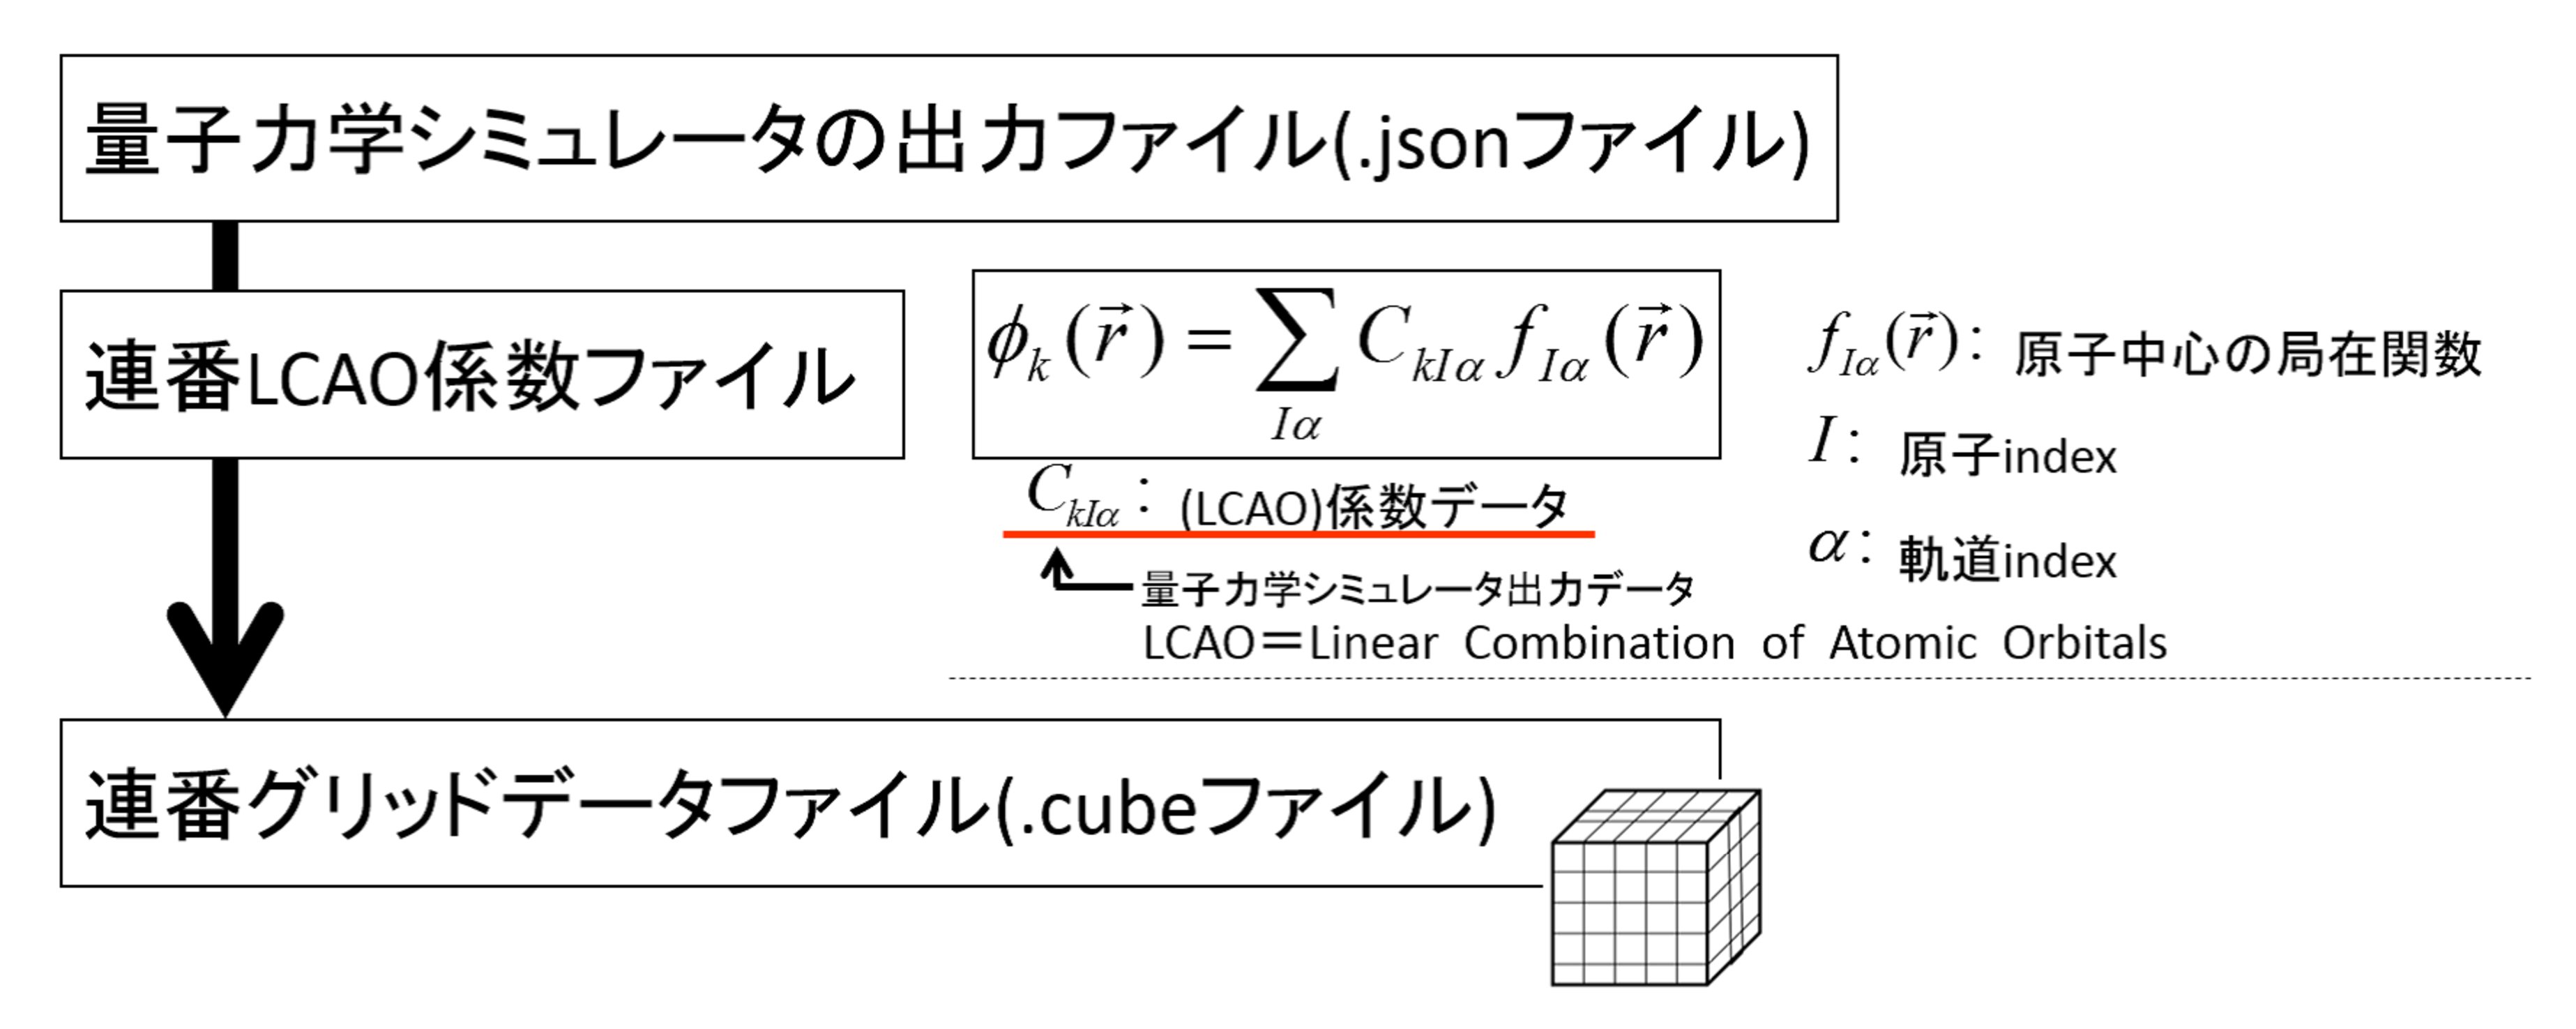
\includegraphics[width=15cm,clip]{fig/workflow.eps}
\caption{Wave Tool のワークフロー}
\label{fig:work flow}
\end{figure}
具体的に行っている作業を簡単に説明すると、
まず量子力学シミュレータの出力ファイル(JSON形式)から、時系列データを取り出している。
次に取り出した時系列データをLCAO係数ファイルへ変換している。
最後にLCAO係数ファイルからelses-generate-cubefile(elsesに付属しているLCAOファイルからCUBEファイルを作成するツール)を使用してCUBEファイルを作成している。

%具体的に行っている作業を簡単に説明すると、
%まず量子力学シミュレータの出力ファイル(JSON形式とXYZ形式)から、時系列データを取り出している。
%次に取り出した時系列データからLCAO係数ファイルを作成している。
%その後、LCAO係数ファイルからelses-generate-cubefile(elsesに付属しているLCAOファイルからCUBEファイルを作成するツール)を使用してrealとimaginaryのCUBEファイルを作成している。
%最後に、realとimaginaryのCUBEファイルからcharge($=\sqrt{\rm{real}^2 + \rm{imaginary}^2}$)のCUBEファイルを作成している。
\begin{figure}[H]
\centering
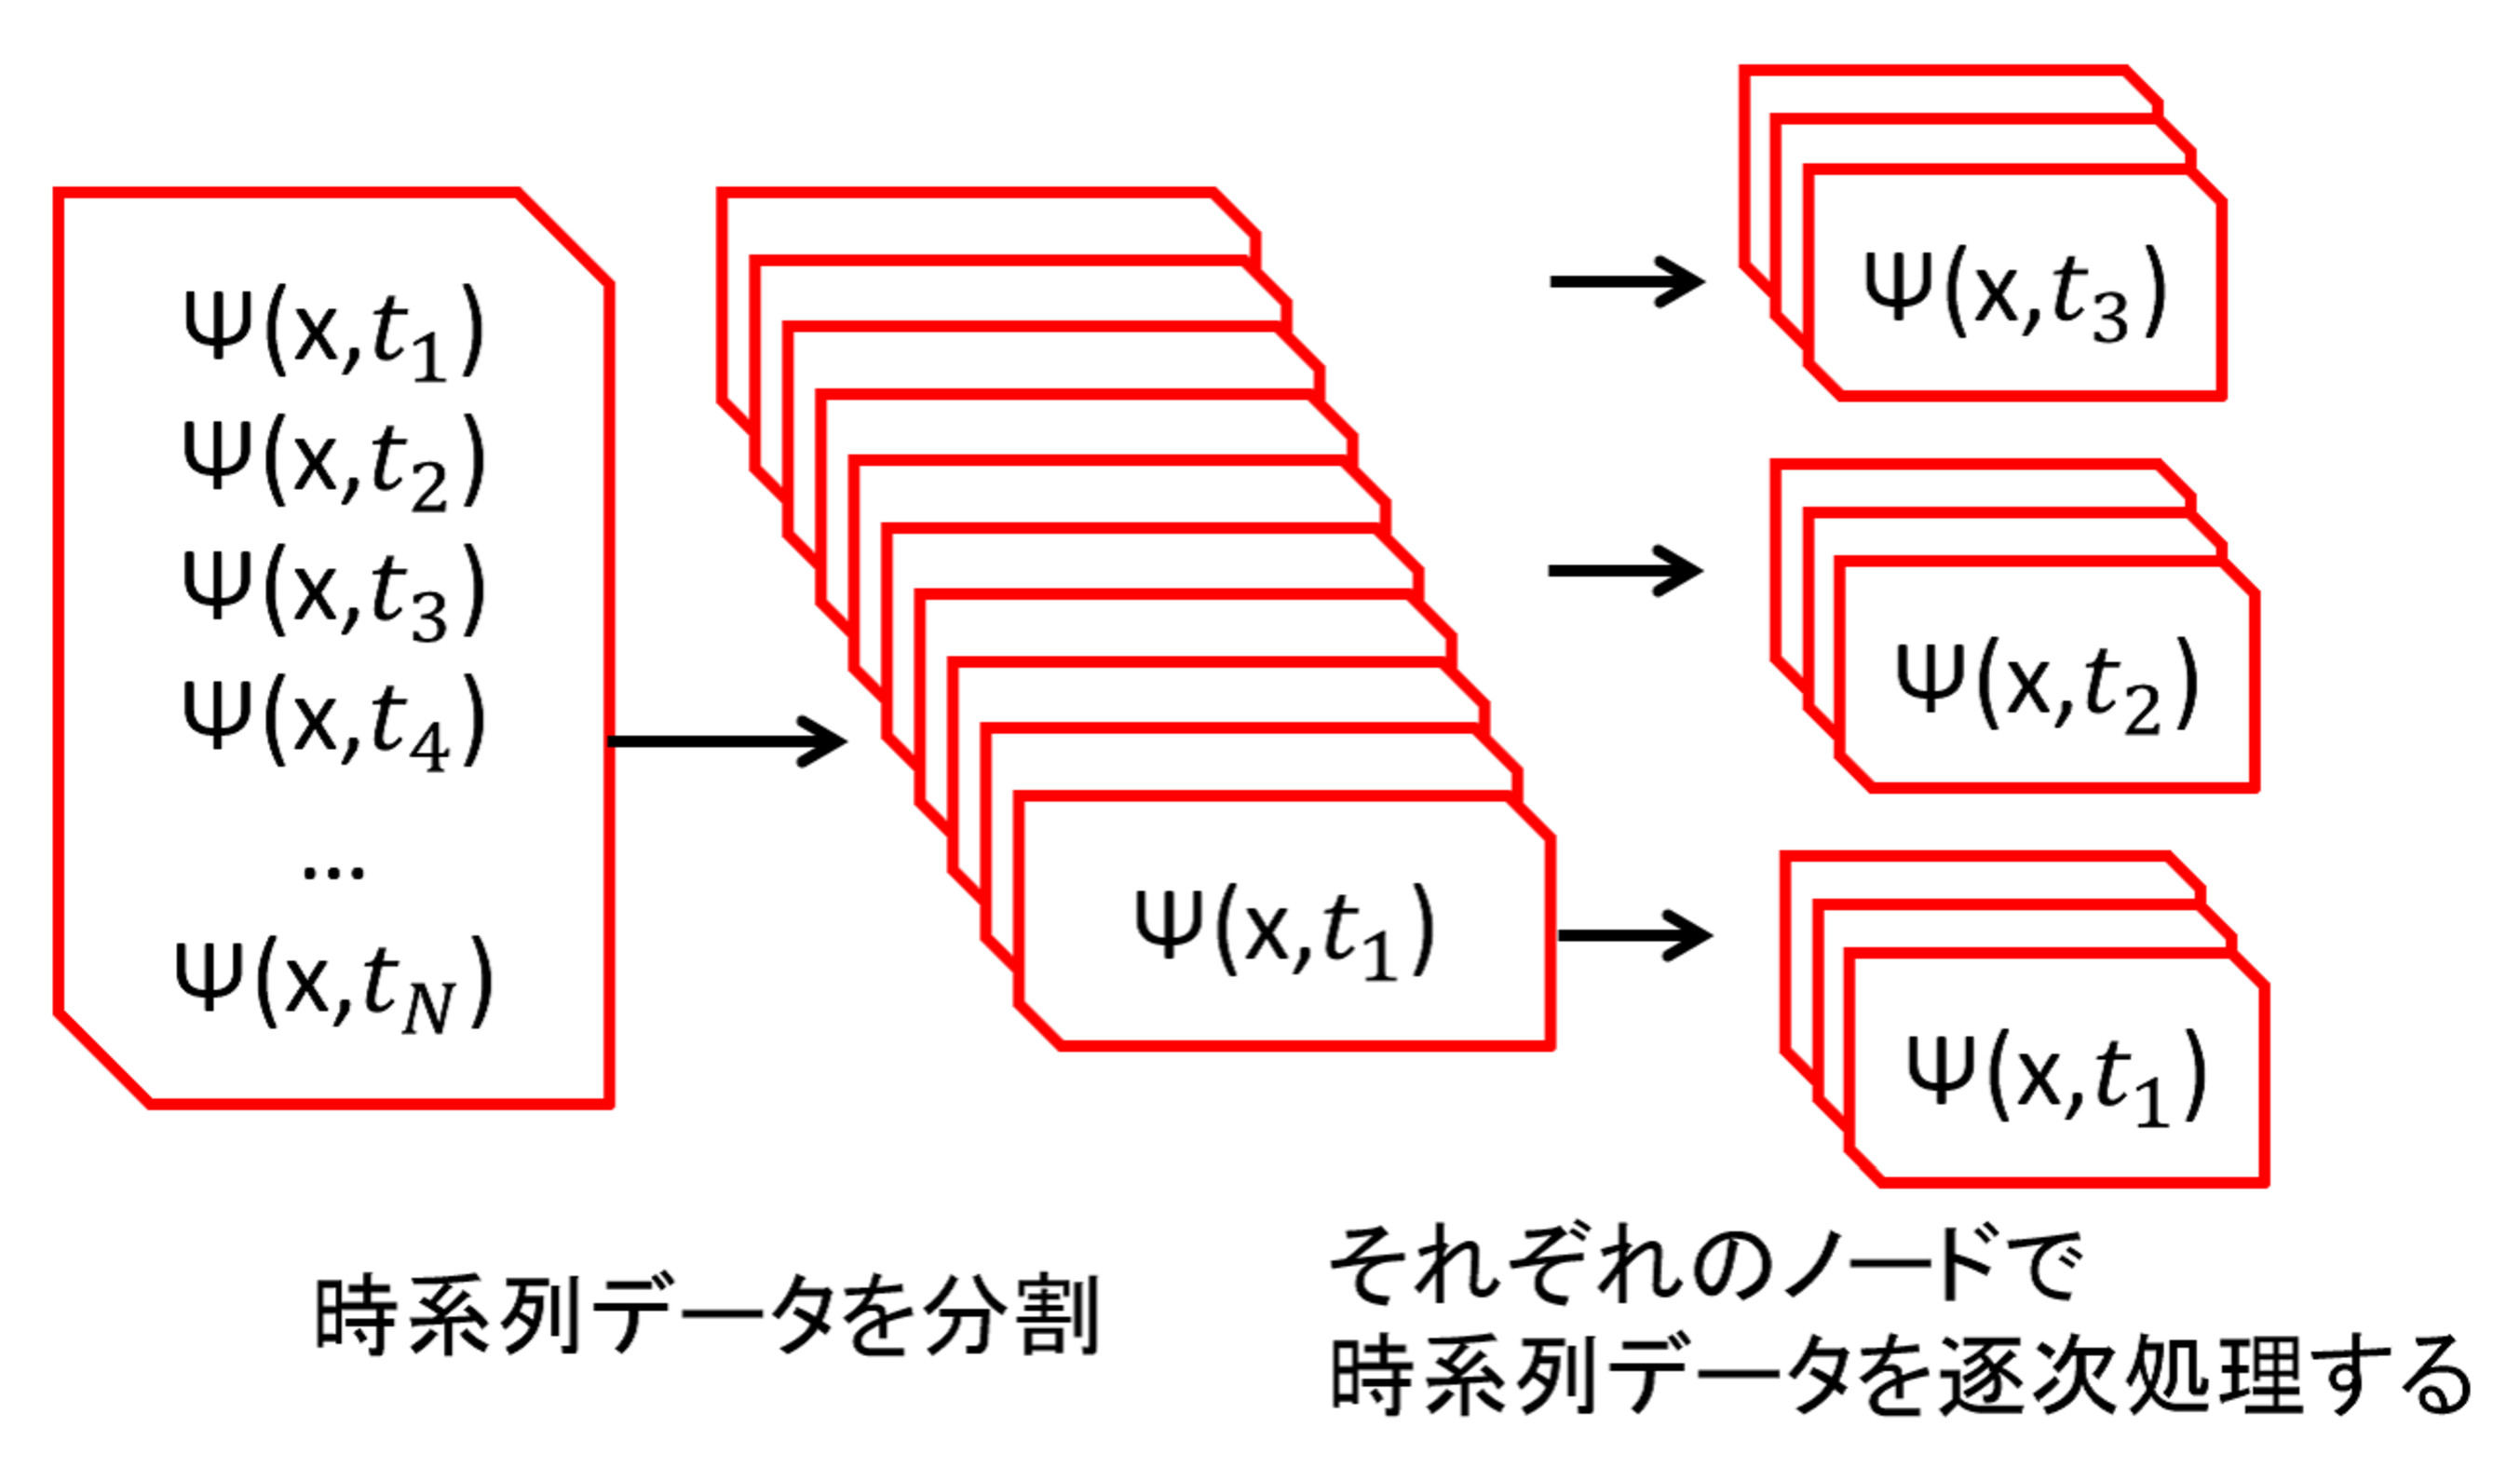
\includegraphics[width=15cm,clip]{fig/work_imag.eps}
\caption{Wave Tool の並列イメージ}
\label{fig:work image}
\end{figure}
主に、並列化が行われている部分はLCAO係数ファイルを作成した後のLCAO係数ファイルからCUBEファイルを作成する部分である。
具体的には、LCAOファイルを作成した後の作業は、1つ1つが完全に独立しているため行う作業を並列数分で分割してそれぞれで逐次処理を行っている。\\
ちなみに、LCAO係数ファイルからCUBEファイルを作成する部分はPythonがfortranのコードを実行して計算を行っている形になっていてfortranのコードがOpenMP並列化されている。

%並列化が行われている部分は、jsonファイルの読み込み部分とLCAO係数ファイルからrealとimaginaryのCUBEファイルを作成する部分、realとimaginaryのCUBEファイルからchargeのCUBEファイルを作成する部分である。\\
%具体的には、
%jsonファイルの読み込み部分では、ファイルが分割で出力されている場合にjsonファイルを並列読み込みするようになっている。
%LCAO係数ファイルからrealとimaginaryのCUBEファイルを作成する部分では、Pythonがfortranのコードを実行して計算を行っている形になっており、fortranのコードがOpenMP並列されている。
%realとimaginaryのCUBEファイルからchargeのCUBEファイルを作成する部分では、作業を並列数分で分割してそれぞれで逐次処理を行っている。

%%%%%%%%%%%%%%%%%%%%%%%%%%%%%%%%%%%%%%%%%%%%%%%%%%%%%%%%%%%%%%%%%%%%%%%%%%%%%%%
\subsection{WaveToolの構成}
%%%%%%%%%%%%%%%%%%%%%%%%%%%%%%%%%%%%%%%%%%%%%%%%%%%%%%%%%%%%%%%%%%%%%%%%%%%%%%%
%\href{https://drive.google.com/file/d/0B8JK8VUUlcKxVF9IRk45RkRXNnM/view?usp=sharing}{WaveTool\_20160121.zip}をダウンロード\\
%WaveTool配布場所(量子ダイナミクス作業ログ(安部))からWaveToolの最新版をダウンロード。

WaveTool\_20170119.zipの展開\\
\begin{Verbatim}[frame=single]
$ unzip WaveTool_20170119.zip
\end{Verbatim}

展開すると、以下の9個のファイルがある。\\
\begin{itemize}
\item Main\_AutoWave.py\\
⇒WaveToolのメインプログラムである。Windows上で実行した場合OSErrorを起こすため、Linux上で実行すること。\\

\item LCAO\_converter.py\\
⇒ELSESのelses-generate-cubefileを利用してCUBEファイルを作成する。\\

\item charge\_makes\_cube.py\\
⇒realのCUBEファイルとimaginaryのCUBEファイルからchargeのCUBEファイルを作成する。\\

\item input\_mesh\_grid\_lib.py\\
⇒input\_mesh\_gridを作成する。\\

\item make\_input\_mesh\_grid\_20151013.py\\
⇒input\_mesh\_gridを自動生成するツール。\\

\item Main\_AutoWave\_not\_LCAO\_20151022.py\\
⇒LCAO係数ファイルを作成せずにcubeファイルを作成するツール。1度cubeファイルを作成した後、meshを変更したくなった場合に使用する。\\

\item charge\_makes\_cube\_dir.py\\
⇒real,imagのcubeファイルがあるときにcharのcubeファイルを作成するツール。\\

\item readme.txt
⇒Wave Toolの使用方法が簡単に書いてある。\\

\item WaveToolManual.pdf(本マニュアル)\\
⇒Wave Toolの仕様などが書いてある。\\

\end{itemize}


%%%%%%%%%%%%%%%%%%%%%%%%%%%%%%%%%%%%%%%%%%%%%%%%%%%%%%%%%%%%%%%%%%%%%%%%%%%%%%%
\subsection{WaveToolの実行}
%%%%%%%%%%%%%%%%%%%%%%%%%%%%%%%%%%%%%%%%%%%%%%%%%%%%%%%%%%%%%%%%%%%%%%%%%%%%%%%

実行コマンドは以下の通りである。\\
注)jsonファイルを分割している場合(-s オプションを使用している場合)は親玉のjsonファイル(数字が書かれていないもの)を入力する\\

\begin{Verbatim}[frame=single]
usage: Main_AutoWave.py [-h] [-s STRIDE] [-load-min LOAD-MIN]
                        [-load-max LOAD-MAX] [-cutoff-au CUTOFF]
                        [-input_mesh_grid PATH] [-alpha ALPHA] [-mesh MESH]
                        [-target target] [-core CORE] [-periodic periodic]
                        [--parallel] [--position] [--LCAO] [--big-endian]
                        elses-generate-cubefile JSON XYZ BASIS
Main_AutoWave.py: error: too few arguments
\end{Verbatim}

エラー無く、実行できると、「***.json.cube」というフォルダが出来上がり、
中に、real、imag、charというフォルダが出来ており、中にCubeファイルが作成されている。\\

オプションの説明\\
\begin{itemize}
\item -h\\
help\\
\item -s STRIDE\\
何個飛ばしで読み込むか(wavepacket内部のステップを割り切れるかどうかで判定している) (default:1)\\
\item -load-min LOAD-MIN\\
読み込むステップの最小値を決めている(default:0)\\
\item -load-max LOAD-MAX\\
読み込むステップの最大値を決めている(default:10000000)\\
\item -cutoff-au CUTOFF\\
elses-generate-cubefileで使用するcutoffの値(default:8.0)\\
\item -input\_mesh\_grid PATH\\
別階層にあるinput\_mesh\_gridを現在のディレクトリに移動する(すでにある場合は何もしない)(自動でinput\_mesh\_gridを作製するオプションと併用した場合はこのオプションは動作しない)\\
\item -alpha ALPHA\\
最初のステップのmeanの値と最後のステップの値の合計のMSDを使用して$mean \pm alpha\sqrt{MSD}$の範囲(正方形)のinput\_mesh\_gridを作製(既にあるinput\_mesh\_gridを上書してしまうので注意)\\
(-\--position と -alphaを同時に使用すると最大でpositionで作製される範囲になるようにalphaで作製される)\\
\item -mesh MESH\\
オプションでinput\_mesh\_gridを作製する際のメッシュ数を変更する(一辺のメッシュ数は大体 長さ[a.u.]*MESH で作製される) default : 1.0\\
\item -target target\\
作りたいwavepacket内部のステップを指定する(-load-min,maxは無視される)(複数ステップを入力する場合は「115,223,587」のように「,」区切りでスペースがないように入力)\\
\item -core CORE\\
-\--parallelを使用したときの並列数を決めている(defaultではOMP\_NUM\_THREADSの値になる。OMP\_NUM\_THREADSがない場合は最大の並列数になる)\\
\item -\--parallel\\
読み込みとcharのcubeファイル作製をpythonで並列化させる(メモリが十分にあるときだけ使用すること)\\
\item -\--position\\
xyzファイルを読み込みその原子が全て含まれるように自動でinput\_mesh\_gridを作製(既にあるinput\_mesh\_gridを上書してしまうので注意)\\
\item -\--big-endian\\
oakleaf,Kでのbynari出力を読み込む時に使用する\\
\item -\--LCAO\\
LCAO係数データファイル(output\_wavefunction)のみを出力するモード(mpi並列で実行しても意味ありません)\\
\end{itemize}

%%%%%%%%%%%%%%%%%%%%%%%%%%%%%%%%%%%%%%%%%%%%%%%%%%%%%%%%%%%%%%%%%%%%%%%%%%%%%%%
\subsubsection{具体例}
%%%%%%%%%%%%%%%%%%%%%%%%%%%%%%%%%%%%%%%%%%%%%%%%%%%%%%%%%%%%%%%%%%%%%%%%%%%%%%%
初めの100ステップ分のCubeファイルを作成する場合
\begin{Verbatim}[frame=single]
$ python Main_AutoWave.py -load-min 0 -load-max 100 \
elses-generate-cubefile out.json position.xyz output_basis_information.txt
\end{Verbatim}
5ステップ刻みでCubeファイルを作成する場合
\begin{Verbatim}[frame=single]
$ python Main_AutoWave.py -s 5 elses-generate-cubefile \
out.json position.xyz output_basis_information.txt
\end{Verbatim}
0,10,100ステップ目のCubeファイルを作成する場合
\begin{Verbatim}[frame=single]
$ python Main_AutoWave.py -target 0,10,100 elses-generate-cubefile \
out.json position.xyz output_basis_information.txt
\end{Verbatim}


%%%%%%%%%%%%%%%%%%%%%%%%%%%%%%%%%%%%%%%%%%%%%%%%%%%%%%%%%%%%%%%%%%%%%%%%%%%%%%%
\subsection{mpi4pyで並列実行する場合}
%%%%%%%%%%%%%%%%%%%%%%%%%%%%%%%%%%%%%%%%%%%%%%%%%%%%%%%%%%%%%%%%%%%%%%%%%%%%%%%
実行方法は、mpi4pyをインストールしている状態で以下のように「python Main\_AutoWave.py」の前に「mpirun -n 4」などと普通のmpiプログラムのように並列数指定して実行する。

実行コマンド
\begin{Verbatim}[frame=single]
$ mpirun -n 4 python Main_AutoWave.py
usage: Main_AutoWave.py [-h] [-s STRIDE] [-load-min LOAD-MIN]
                        [-load-max LOAD-MAX] [-cutoff-au CUTOFF]
                        [-input_mesh_grid PATH] [-alpha ALPHA] [-mesh MESH]
                        [-target target] [-core CORE] [--parallel]
                        [--position] [--big-endian]
                        elses-generate-cubefile JSON XYZ BASIS
Main_AutoWave.py: error: too few arguments
\end{Verbatim}
オプションについては普通に実行する場合と同様

%%%%%%%%%%%%%%%%%%%%%%%%%%%%%%%%%%%%%%%%%%%%%%%%%%%%%%%%%%%%%%%%%%%%%%%%%%%%%%%
\subsubsection{具体例}
%%%%%%%%%%%%%%%%%%%%%%%%%%%%%%%%%%%%%%%%%%%%%%%%%%%%%%%%%%%%%%%%%%%%%%%%%%%%%%%
初めの100ステップ分のCubeファイルを作成する場合
\begin{Verbatim}[frame=single]
$ mpirun -n 4 python Main_AutoWave.py -load-min 0 -load-max 100 \
elses-generate-cubefile out.json position.xyz output_basis_information.txt
\end{Verbatim}
5ステップ刻みでCubeファイルを作成する場合
\begin{Verbatim}[frame=single]
$ mpirun -n 4 python Main_AutoWave.py -s 5 elses-generate-cubefile \
out.json position.xyz output_basis_information.txt
\end{Verbatim}

%%%%%%%%%%%%%%%%%%%%%%%%%%%%%%%%%%%%%%%%%%%%%%%%%%%%%%%%%%%%%%%%%%%%%%%%%%%%%%%
\subsection{並列性能の結果}
%%%%%%%%%%%%%%%%%%%%%%%%%%%%%%%%%%%%%%%%%%%%%%%%%%%%%%%%%%%%%%%%%%%%%%%%%%%%%%%
mpi4pyを使用したWaveToolの並列化を行った部分の並列性能についてベンチマークを取った。使用した環境は、京都大学のスパコン(laurel)と東京大学のスパコン(oakleaf FX10)。
結果として、ノード数を2,4,8,…倍と上げていくと計算時間が短縮されるのを確認できた。

\begin{table}[H]
  \centering
  \caption{laurelでのWaveToolの並列化を行った部分の実行時間データ}
  \label{table:pi-02}
\begin{comment}
  \begin{tabular}{|c|c|} \hline
   1 & 1911.592165 \\ \hline
   2 & 1011.976167 \\ \hline
   4 & 546.830317 \\ \hline
   8 & 327.062007 \\ \hline
  16 & 222.988008 \\ \hline
  \end{tabular}
\end{comment}
  \begin{tabular}{|c|c|} \hline
   ノード数N & 実行時間T(s) \\ \hline
   1 & 1579.838029 \\ \hline
   2 & 800.036737 \\ \hline
   4 & 399.55529 \\ \hline
   8 & 200.265127 \\ \hline
  16 & 104.539619 \\ \hline
  \end{tabular}
\end{table}

\begin{figure}[H]
\centering
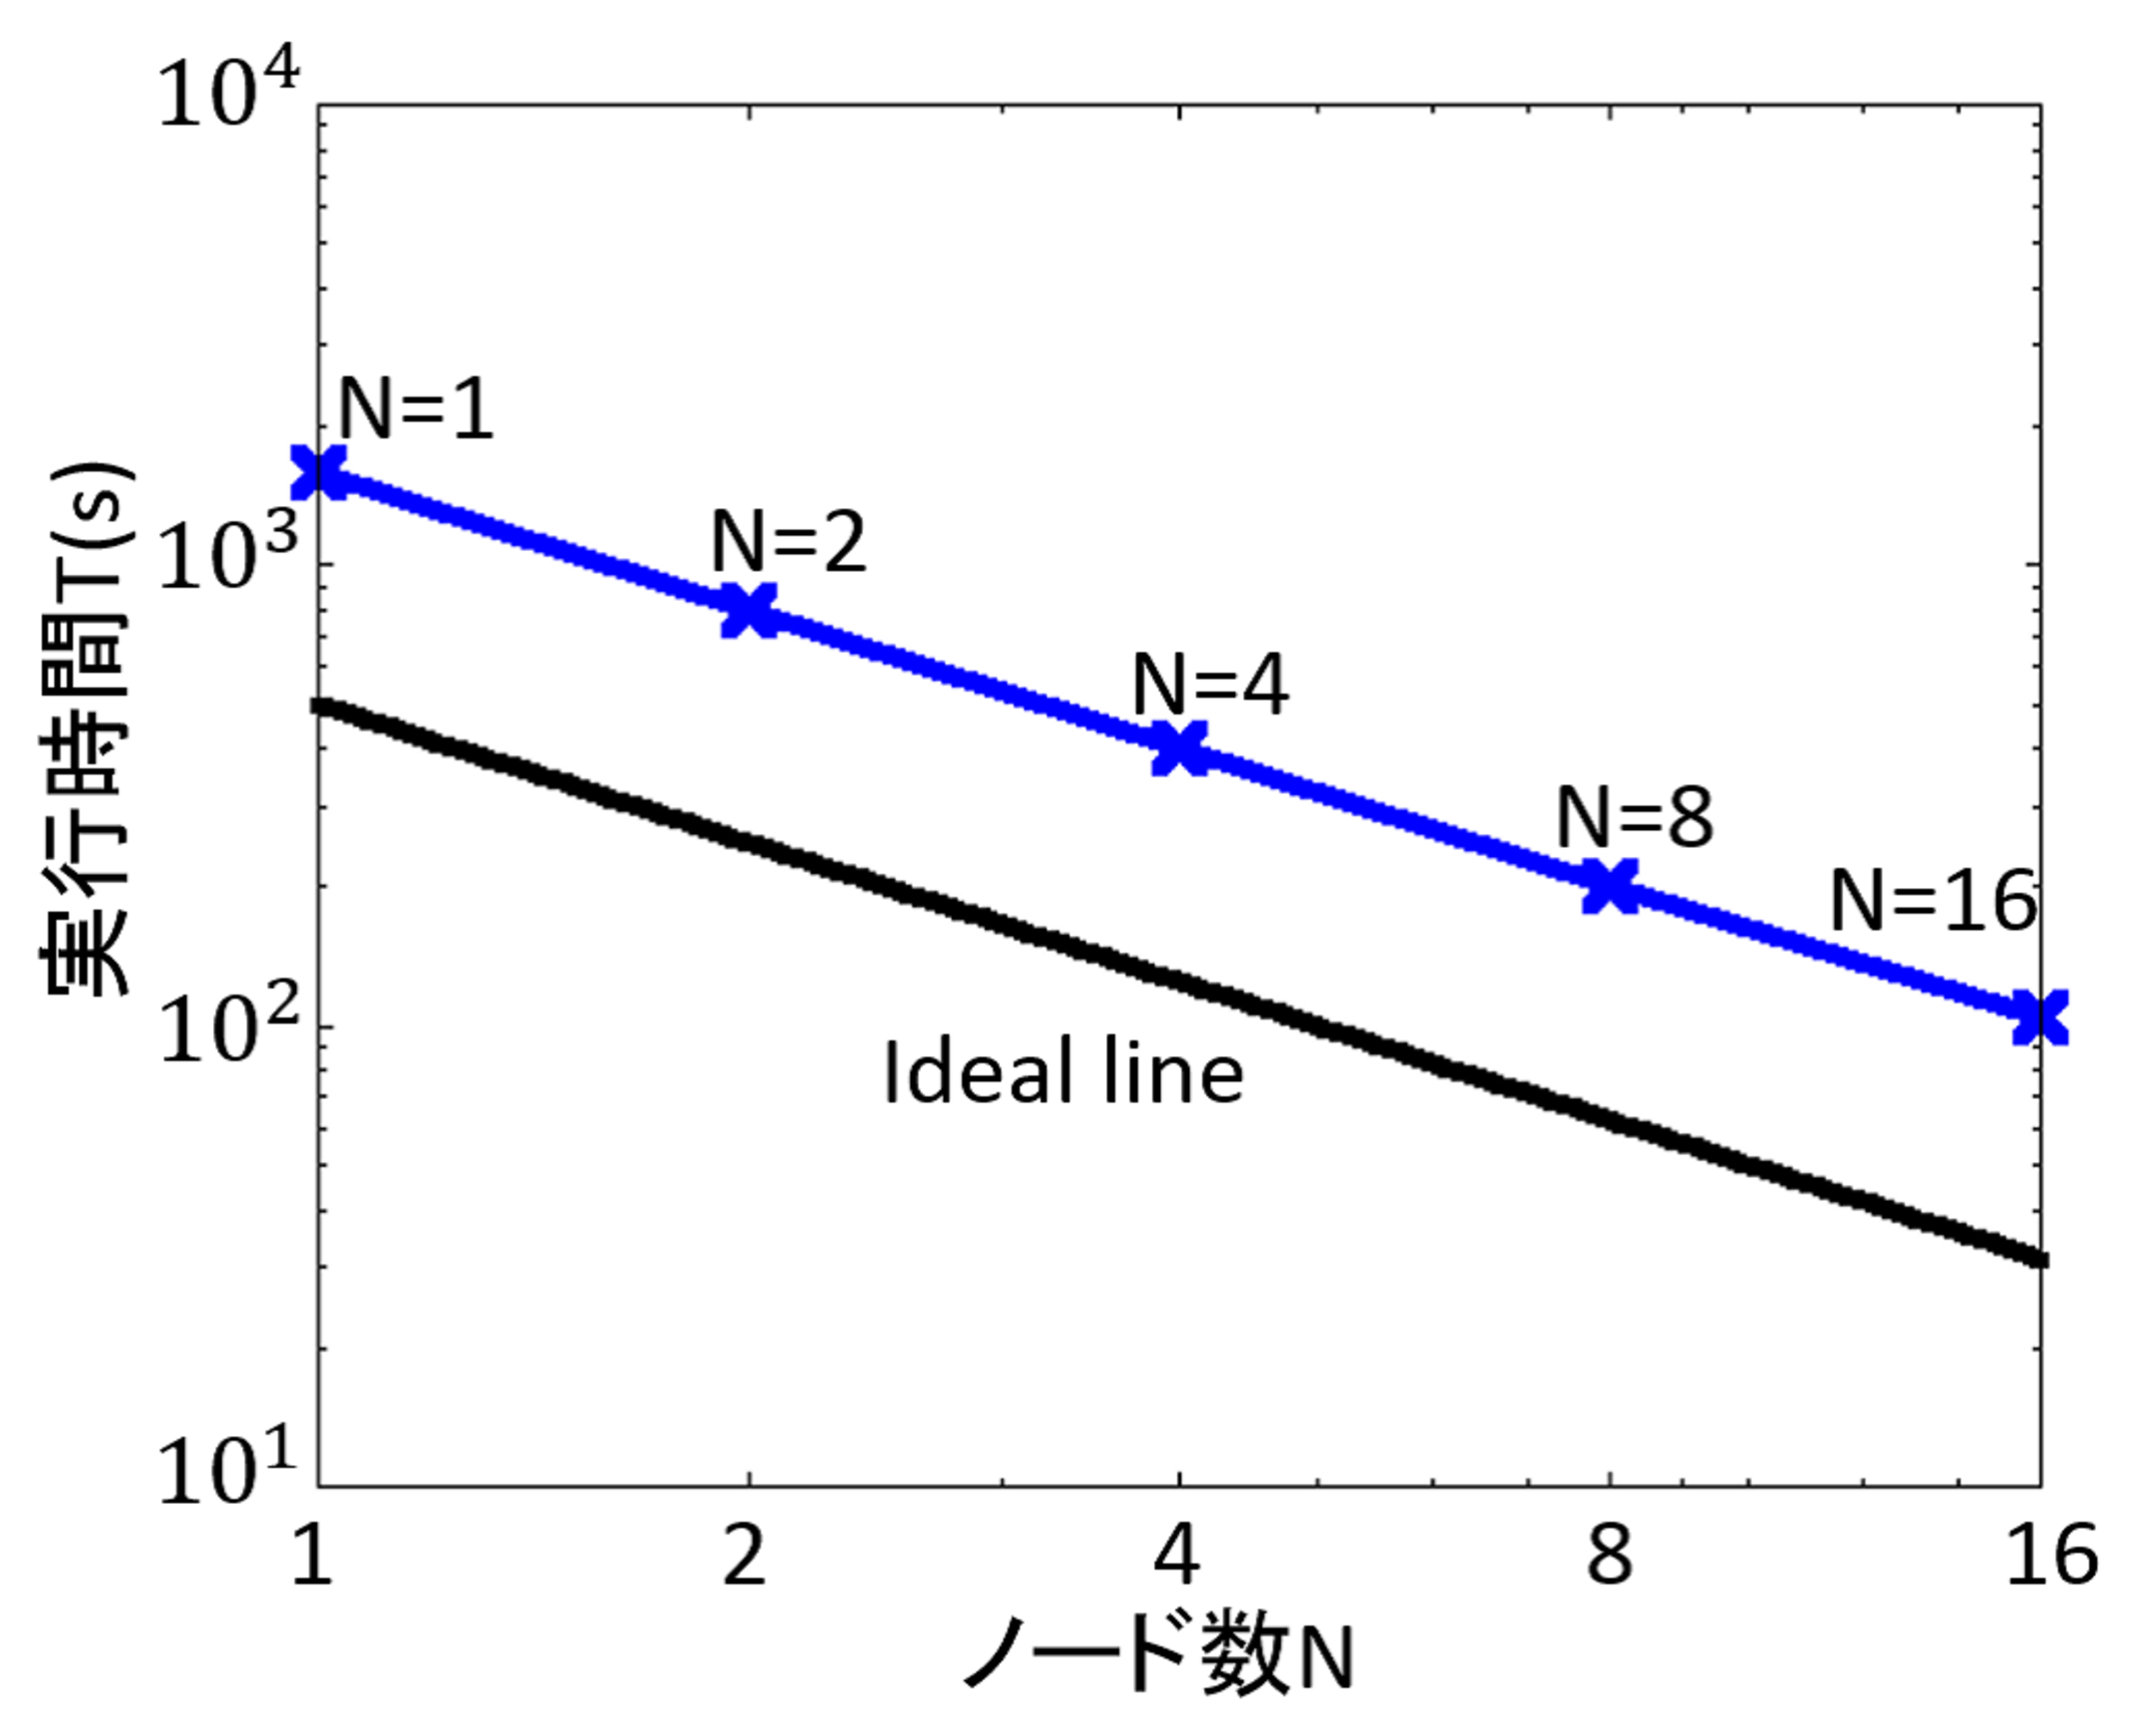
\includegraphics[width=9cm,clip]{fig/laurel_WaveTool.eps}
\caption{laurelでのWaveToolの並列化を行った部分の並列効率。}
\label{fig:pi-01}
\end{figure}

\begin{table}[H]
  \centering
  \caption{Oakleaf FX10でのWaveToolの並列化を行った部分の実行時間データ}
  \label{table:pi-02}
\begin{comment}
  \begin{tabular}{|c|c|} \hline
   1 & 5828.75918 \\ \hline
   2 & 3315.157952 \\ \hline
   4 & 2060.418457 \\ \hline
   8 & 1434.50201 \\ \hline
  16 & 1261.334071 \\ \hline
  \end{tabular}
\end{comment}
  \begin{tabular}{|c|c|} \hline
   ノード数N & 実行時間T(s) \\ \hline
   1 & 2670.982229 \\ \hline
   2 & 1334.658283 \\ \hline
   4 & 668.098373 \\ \hline
   8 & 333.59436 \\ \hline
  16 & 174.566309 \\ \hline
  \end{tabular}
\end{table}

\begin{figure}[H]
\centering
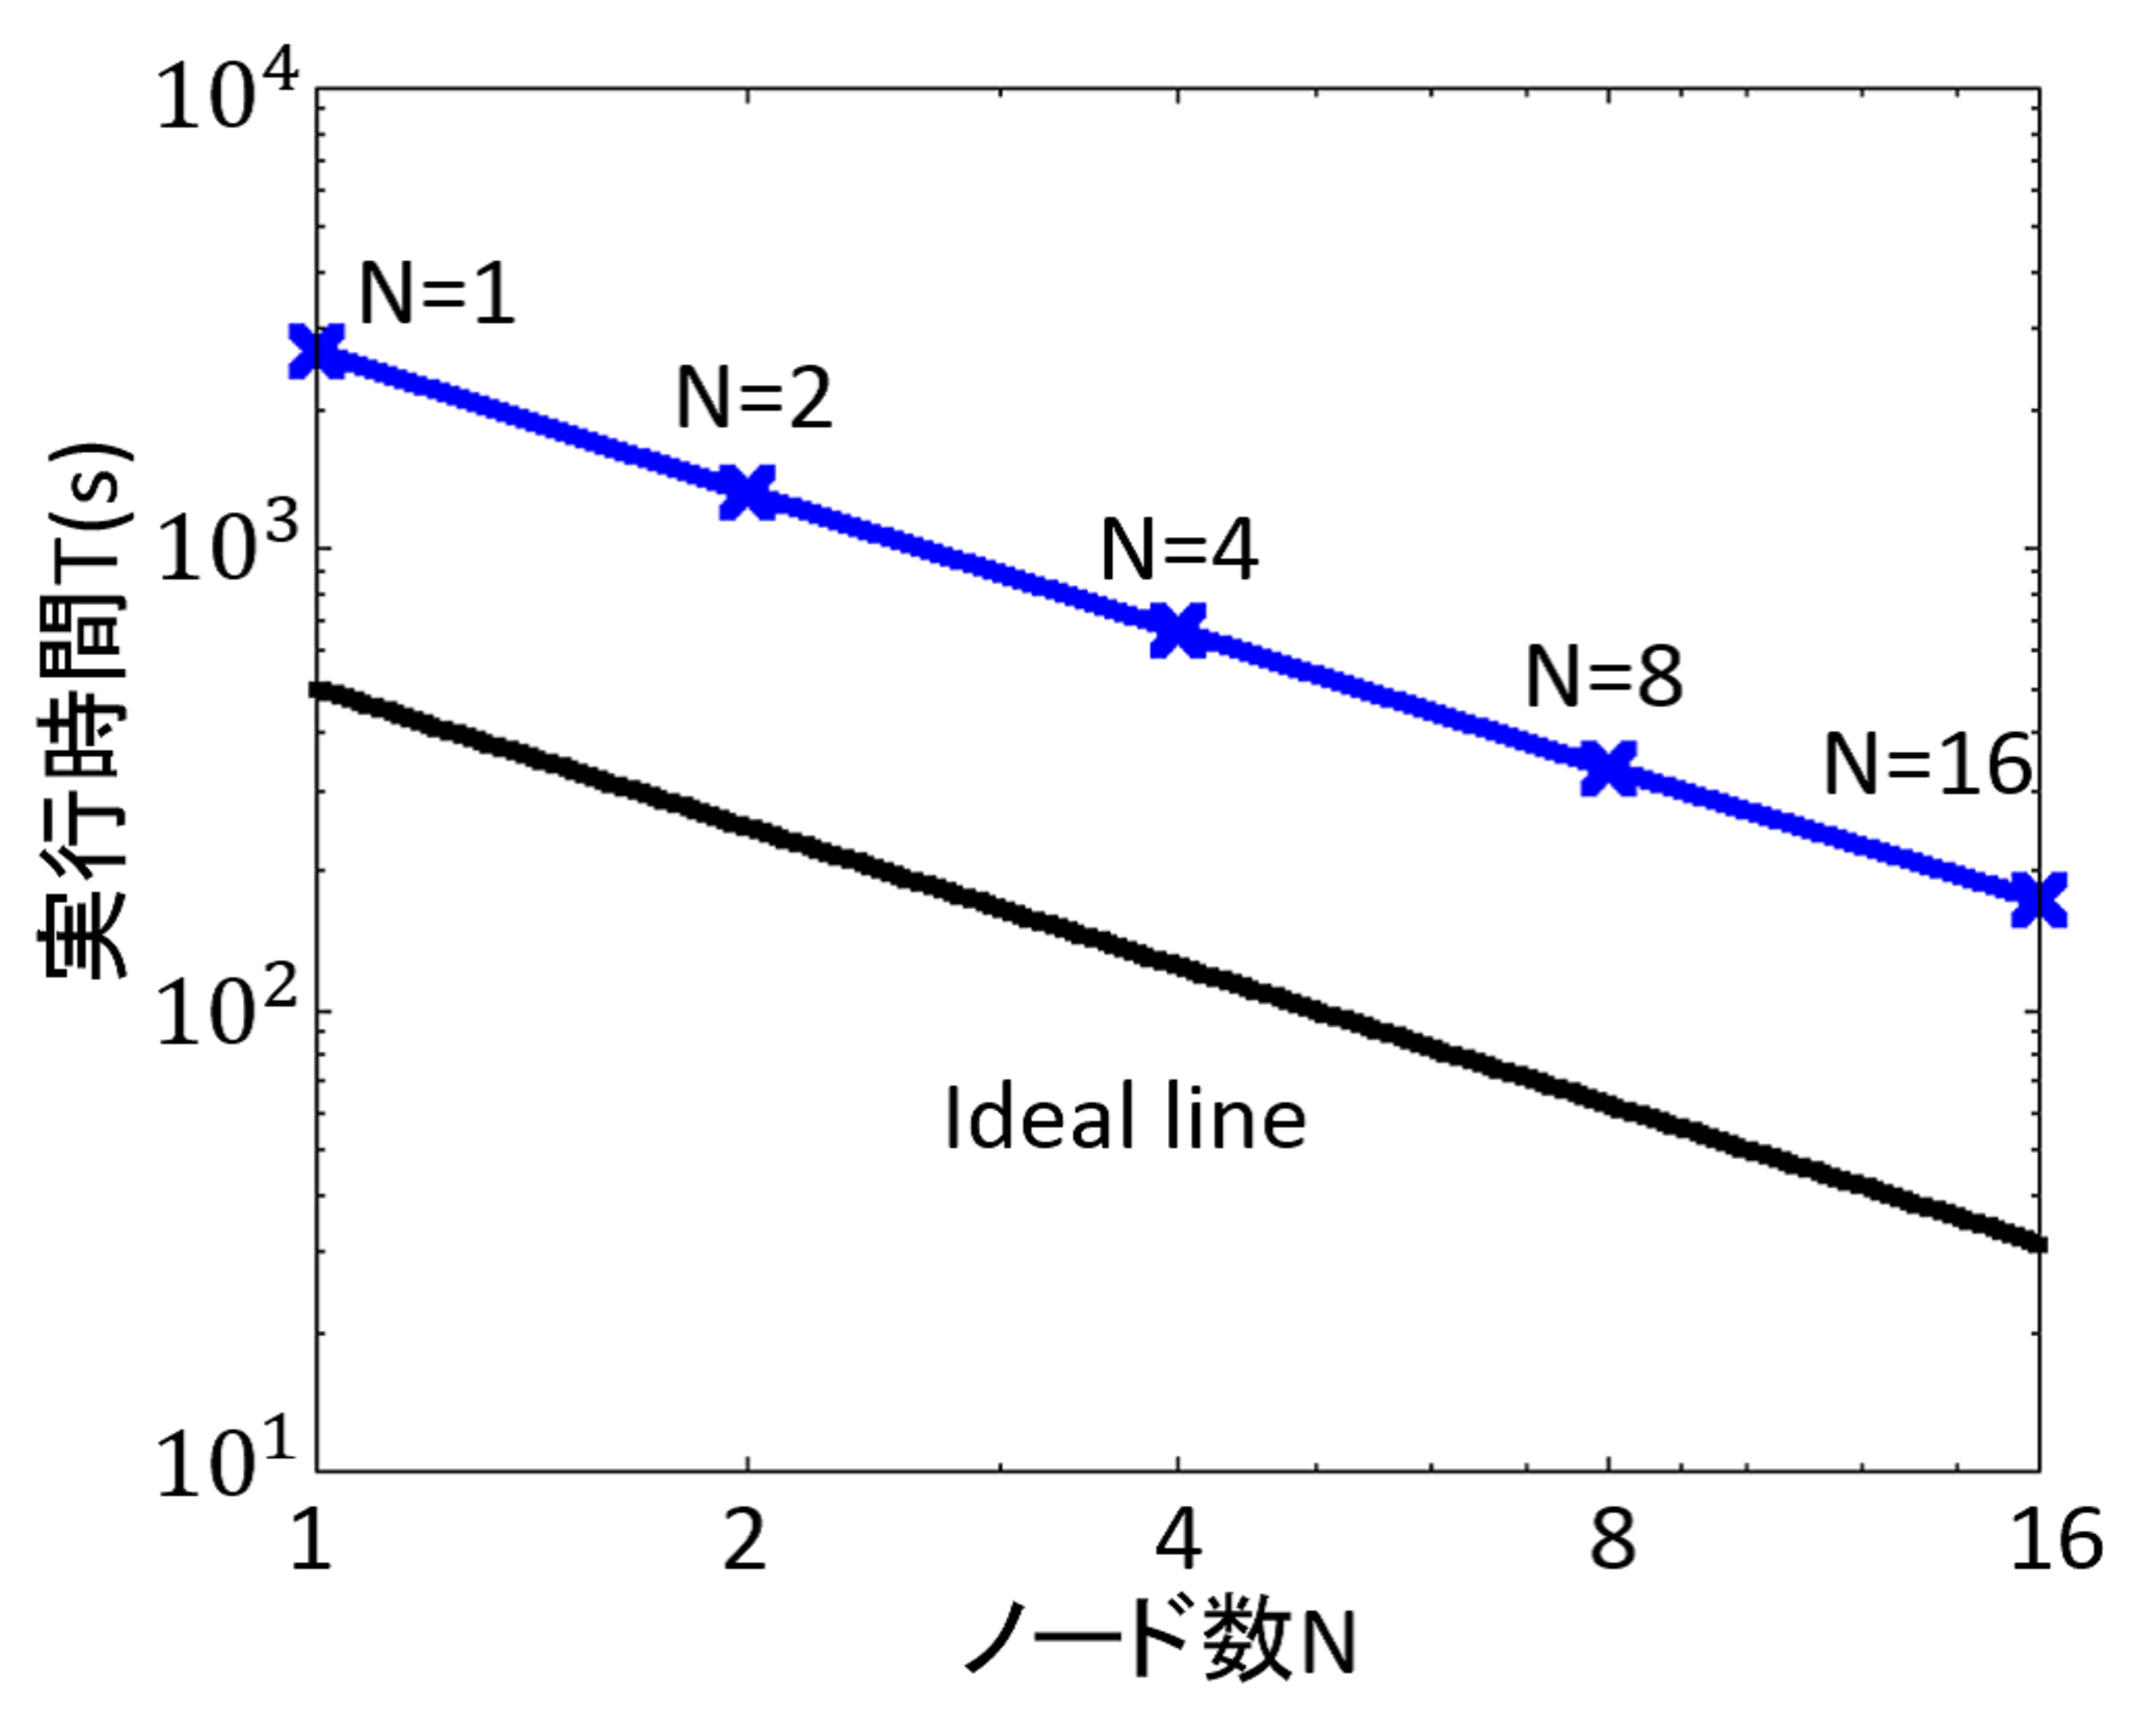
\includegraphics[width=9cm,clip]{fig/oakleaf_WaveTool.eps}
\caption{Oakleaf FX10でのWaveToolの並列化を行った部分の並列効率。}
\label{fig:pi-01}
\end{figure}

%%%%%%%%%%%%%%%%%%%%%%%%%%%%%%%%%%%%%%%%%%%%%%%%%%%%%%%%%%%%%%%%%%%%%%%%%%%%%%%
\subsection{残りのツールについて}
%%%%%%%%%%%%%%%%%%%%%%%%%%%%%%%%%%%%%%%%%%%%%%%%%%%%%%%%%%%%%%%%%%%%%%%%%%%%%%%

%%%%%%%%%%%%%%%%%%%%%%%%%%%%%%%%%%%%%%%%%%%%%%%%%%%%%%%%%%%%%%%%%%%%%%%%%%%%%%%
\subsubsection{make\_input\_mesh\_grid\_20151013.py}
%%%%%%%%%%%%%%%%%%%%%%%%%%%%%%%%%%%%%%%%%%%%%%%%%%%%%%%%%%%%%%%%%%%%%%%%%%%%%%%
input\_mesh\_gridを自動生成するツール。\\

実行コマンド
\begin{Verbatim}[frame=single]
>python make_input_mesh_grid_20151013.py
usage: make_input_mesh_grid_20151013.py [-h] [-group GROUP]
                                        [-group-min GROUP-MIN]
                                        [-group-max GROUP-MAX]
                                        [-cutoff-au CUTOFF] [-mesh MESH]
                                        XYZ
make_input_mesh_grid_20151013.py: error: too few arguments
\end{Verbatim}

オプションの説明
\begin{itemize}
\item -group GROUP\\
group idを読み込み、原子にgroup idを割り振る。(defaultは、一原子一グループでxyzファイルに書かれている順番でグループが割り当てられる。)
\item -group-min GROUP-MIN\\
作成する範囲に入れるグループの最低値を決めている。default : 1
\item -group-max GROUP-MAX\\
作成する範囲に入れるグループの最大値を決めている。default : 10000000
\item -cutoff-au CUTOFF\\
一番端の原子からどのくらいの距離を離すか決めている。単位は[a.u.]。default : 8.0
\item -mesh MESH\\
メッシュ数を変更する(一辺のメッシュ数は大体 長さ[a.u.]*MESH で作製される) default : 1.0\\
\end{itemize}

具体例\\
45から55番目のグループの場所にinput\_mesh\_grid.txtを合わせたい場合
\begin{Verbatim}[frame=single]
$ python make_input_mesh_grid_20151013.py -group group_id.txt \
-group-min 45 -group-max 55 position.xyz
\end{Verbatim}


%%%%%%%%%%%%%%%%%%%%%%%%%%%%%%%%%%%%%%%%%%%%%%%%%%%%%%%%%%%%%%%%%%%%%%%%%%%%%%%
\subsubsection{Main\_AutoWave\_not\_LCAO\_20151022.py}
%%%%%%%%%%%%%%%%%%%%%%%%%%%%%%%%%%%%%%%%%%%%%%%%%%%%%%%%%%%%%%%%%%%%%%%%%%%%%%%
LCAO係数ファイルを作成せずにcubeファイルを作成するツール。1度cubeファイルを作成した後、meshを変更したくなった場合に使用する。\\
\begin{Verbatim}[frame=single]
>python Main_AutoWave_not_LCAO_20151022.py
usage: Main_AutoWave_not_LCAO_20151022.py [-h] [-s STRIDE] [-cutoff-au CUTOFF]
                                          [-input_mesh_grid PATH]
                                          [-position PATH] [-mesh MESH]
                                          [--parallel]
                                          elses-generate-cubefile basis_dir
Main_AutoWave_not_LCAO_20151022.py: error: too few arguments
\end{Verbatim}
basis\_dirには、「*.json.cube/」を入力する。\\

オプションの説明
\begin{itemize}
\item -position PATH\\
PATHにxyzファイルを入力するとそのxyzファイルの原子がすべて入るように自動でinput\_mesh\_grig.txtを作成する。\\
\item 残りのオプションはMain\_AutoWave.pyと同じ。
\end{itemize}

具体例\\
meshの位置を作り直す場合
\begin{Verbatim}[frame=single]
$ python make_input_mesh_grid_20151013.py -group group_id.txt \
-group-min 45 -group-max 55 position.xyz
$ python Main_AutoWave_not_LCAO_20151022.py \
elses-generate-cubefile out.json.cube/
\end{Verbatim}

meshの数を増やす場合
\begin{Verbatim}[frame=single]
$ python Main_AutoWave_not_LCAO_20151022.py -position position.xyz \
-mesh 2.0 elses-generate-cubefile out.json.cube/
\end{Verbatim}

%%%%%%%%%%%%%%%%%%%%%%%%%%%%%%%%%%%%%%%%%%%%%%%%%%%%%%%%%%%%%%%%%%%%%%%%%%%%%%%
\subsubsection{charge\_makes\_cube\_dir.py}
%%%%%%%%%%%%%%%%%%%%%%%%%%%%%%%%%%%%%%%%%%%%%%%%%%%%%%%%%%%%%%%%%%%%%%%%%%%%%%%
real,imagのcubeファイルがあるときにcharのcubeファイルを作成するツール。\\
$<$dir$>$に*.json.cubeを指定すると*.json.cubeの中にcharというフォルダを作成して*.json.cubeの中にあるreal,imagのフォルダの中にあるファイルからcharを作成する。
\begin{Verbatim}[frame=single]
>python charge_makes_cube_dir.py
Usage: python charge_makes_cube.py <dir> [parallel]
\end{Verbatim}
第3引数に「parallel」を入力すると並列化されます。

具体例\\
\begin{Verbatim}[frame=single]
$ python charge_makes_cube.py out.json.cube parallel
\end{Verbatim}

%%%%%%%%%%%%%%%%%%%%%%%%%%%%%%%%%%%%%%%%%%%%%%%%%%%%%%%%%%%%%%%%%%%%%%%%%%%%%%%
\subsubsection{CUBE→pngへのバッチ処理によるグリッド可視化}
%%%%%%%%%%%%%%%%%%%%%%%%%%%%%%%%%%%%%%%%%%%%%%%%%%%%%%%%%%%%%%%%%%%%%%%%%%%%%%%
VisBAR WBのマニュアルを参照

%%%%%%%%%%%%%%%%%%%%%%%%%%%%%%%%%%%%%%%%%%%%%%%%%%%%%%%%%%%%%%%%%%%%%%%%%%%%%%%
\subsubsection{連番png→gif動画の生成}
%%%%%%%%%%%%%%%%%%%%%%%%%%%%%%%%%%%%%%%%%%%%%%%%%%%%%%%%%%%%%%%%%%%%%%%%%%%%%%%
VisBAR ITのマニュアルを参照


\newpage
\appendix
\section{更新履歴}
\begin{itemize}
\item 初稿 2016/09/08
\item 引数にbasis infomationを追加 2016/09/08

\end{itemize}
\end{document}
